\usepackage{graphicx}
\usepackage{rotating}
\usepackage{hyperref}
\usepackage{caption}
\usepackage[normalem]{ulem}
\usepackage{wasysym}
\usepackage{amsmath}
\usepackage{caption}
\usepackage[utf8]{inputenc}
\usepackage[english]{babel}
\usepackage{pifont}


\usepackage[style=authoryear,sorting=ynt]{biblatex}
\usepackage[font={small}]{caption}

\captionsetup[figure]{labelformat=empty}% redefines the caption setup of the figures environment in the beamer class.
\usepackage{caption}
\captionsetup[figure]{font=tiny}

\setbeamertemplate{navigation symbols}{}
\setbeamertemplate{title page}[empty]

\setbeamerfont{subtitle}{size=\small}

\setbeamercovered{transparent}

\definecolor{BaptisteBlue}{HTML}{6495ED}
\definecolor{SurveyBlue}{HTML}{619CFF}
\definecolor{BaptisteOrange}{HTML}{F39C12}
\definecolor{BaptisteGreen}{HTML}{1E8449}
\definecolor{BaptisteLightGreen}{HTML}{28B463}
\definecolor{BaptisteGrey}{HTML}{A6ACAF}
\definecolor{BaptisteRed}{HTML}{FF2A2A}
\definecolor{BaptisteBrown}{HTML}{D45500}
\definecolor{BaptisteDarkGrey}{HTML}{8C9193}


\titlegraphic{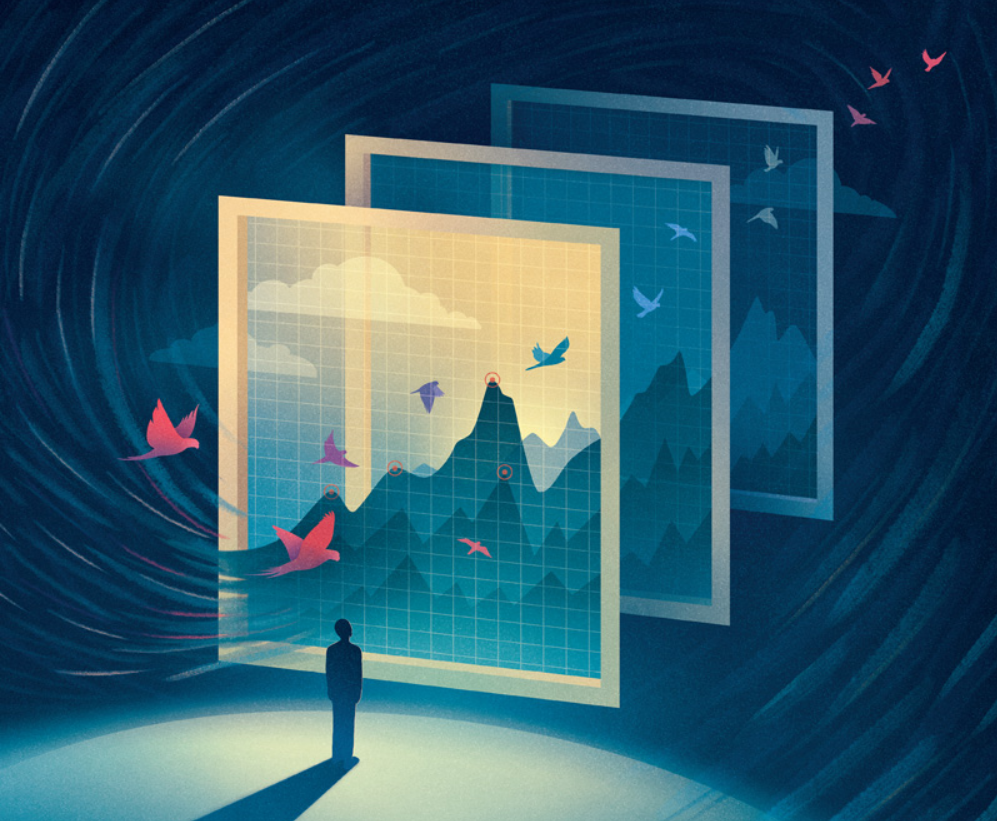
\includegraphics[width=\textwidth,height=.4\textheight]{"images/couv.png"}}

\AtBeginDocument{\title[Spatial and spatio-temporal statistics]{Spatial and spatio-temporal statistics for ecology}}

\let\Tiny=\tiny

\AtBeginPart{}
\AtBeginSubsection{}
\AtBeginSubsubsection{}
\setlength{\emergencystretch}{0em}
\setlength{\parskip}{0pt}